\documentclass[11pt]{article}
\usepackage[utf8]{inputenc}
\usepackage[brazil]{babel}
\usepackage[a4paper,margin=2.3cm]{geometry}
\usepackage{graphicx}
\usepackage{booktabs}
\usepackage{float}
\usepackage{xcolor}
\usepackage{enumitem}
\usepackage[colorlinks=true,linkcolor=blue!60!black,urlcolor=blue!60!black]{hyperref}
\usepackage{titlesec}

\definecolor{ok}{HTML}{2E7D32}
\definecolor{no}{HTML}{C62828}
\newcommand{\ok}{\textcolor{ok}{\textbf{✓}}}
\newcommand{\no}{\textcolor{no}{\textbf{✗}}}

\titleformat{\section}{\large\bfseries\color{blue!50!black}}{\thesection}{0.6em}{}

\title{\textbf{Relatório Completo de Desenvolvimento}\\[4pt]
\large Informação de Domínio na Meta-Aprendizagem para Seleção de Algoritmos:\\
da Hipótese a um Resultado Positivo Validado}
\author{Linha do tempo completa do projeto --- documento para apresentação}
\date{\today}

\begin{document}
\maketitle

\begin{abstract}
\noindent\textbf{Pergunta:} o domínio de um dataset (saúde, finanças, biologia,
imagem, etc.) ajuda a escolher o melhor algoritmo de classificação, além das
meta-features estatísticas? \textbf{Resposta: sim --- de forma pequena, porém real
e validada.} Com \emph{codificação supervisionada por rank médio}, o domínio
melhora a \textbf{acurácia em +1,19 p.p.} e o \textbf{F1-macro em +0,69 p.p.}
(ambas $p<0,001$, positivas em 24 de 30 sementes), em \textbf{547 datasets sem
viés}, sob validação cruzada agrupada (livre de vazamento). Chegamos a esse
resultado após descartar rigorosamente os artefatos que enganam estudos ingênuos e
testar exaustivamente dezenas de abordagens. Este relatório documenta toda essa
jornada, em ordem cronológica.
\end{abstract}

\tableofcontents
\vspace{4pt}\hrule

\section{Objetivo e hipótese}
\textbf{Hipótese central:} o domínio de aplicação de um dataset carrega sinal
preditivo sobre qual algoritmo tende a ser melhor, \emph{além} do já capturado
pelas meta-features estatísticas. \textbf{Restrição:} as meta-features
estatísticas nunca são alteradas; o domínio é sempre \emph{adicionado}.
\textbf{Intuição (confirmada):} certos domínios favorecem certas famílias de
algoritmo (imagem/alta dimensão $\rightarrow$ MLP/SVM; tabular $\rightarrow$
árvores/lineares). O desafio foi \textbf{medir esse sinal sem ser enganado por
ruído}.

\section{Linha do tempo (visão geral)}
\begin{enumerate}[leftmargin=2.2em]
  \item[\textbf{F1.}] Base inicial (116 datasets, 3 algoritmos) e primeiros resultados ``promissores''.
  \item[\textbf{F2.}] A desconfiança: investigação e descarte de \textbf{4 artefatos}.
  \item[\textbf{F3.}] Construção de uma base \textbf{robusta e sem viés} (547 datasets).
  \item[\textbf{F4.}] Descoberta do \textbf{ruído do alvo} (margens $\sim$0,8 p.p.; 26\% de rótulos instáveis).
  \item[\textbf{F5.}] \textbf{Tudo que testamos} --- dezenas de abordagens, a maioria sem ganho.
  \item[\textbf{F6.}] A descoberta: \textbf{target encoding} (codificação supervisionada).
  \item[\textbf{F7.}] Refinamento: a codificação por \textbf{rank médio} é a melhor.
  \item[\textbf{F8.}] \textbf{Resultado final validado} + resultado de sistema.
\end{enumerate}

\section{F1 --- Base inicial e primeiros resultados}
A primeira versão usava \textbf{116 datasets}, pré-selecionados por exigir
palavra-chave de domínio no nome, e \textbf{3 algoritmos} (DecisionTree,
LogisticRegression, Perceptron), com validação cruzada de \textbf{semente única}.
Os resultados pareciam confirmar a hipótese: adicionar texto + domínio elevava o
F1-macro de $\sim$39,9\% para 43,8\%, chegando a 50,2\% ao trocar o modelo por
Gradient Boosting com \emph{tuning}. \textbf{Esses números motivaram o estudo ---
e, depois, a investigação que revelou que boa parte deles eram artefatos.}

\section{F2 --- A desconfiança: descarte de artefatos}
Sob validação rigorosa, os ganhos grandes se decompuseram em \textbf{quatro
artefatos}, cada um isolado e documentado (Tabela~\ref{tab:art}).

\begin{table}[H]\centering
\caption{Artefatos que inflam estudos ingênuos e seu efeito após controle.}
\label{tab:art}
\begin{tabular}{lll}
\toprule
Artefato & Evidência & Após controle \\
\midrule
Semente única & ``+6,5 p.p.'' $\rightarrow$ +1--2 p.p. (CV repetida) & inflado \\
Vazamento textual & TF-IDF cru: +1,7 p.p. (aleatória) $\rightarrow$ $-$1 p.p. (agrupada) & desaparece \\
Confundimento & \texttt{domain\_score} $\leftrightarrow$ nº atributos: $\rho=+0{,}40$ & proxy de dimensão \\
Troca de modelo & baseline+GB iguala o ``campeão'' & era upgrade de modelo \\
\bottomrule
\end{tabular}
\end{table}

\noindent O vazamento foi demonstrado diretamente: o TF-IDF cru \emph{ajuda} sob CV
aleatória, mas o ganho \emph{some} sob CV agrupada por similaridade de colunas ---
prova de que era \textbf{memorização de famílias quase-duplicadas}, não
conhecimento generalizável.

\section{F3 --- Construção da base robusta (547 datasets)}
A base de 116 tinha \textbf{viés de seleção} (só datasets com domínio no nome).
Reconstruímos a partir de todo o OpenML, com filtro técnico de qualidade e
deduplicação por família + tamanho (Figura~\ref{fig:base}).

\begin{figure}[H]\centering
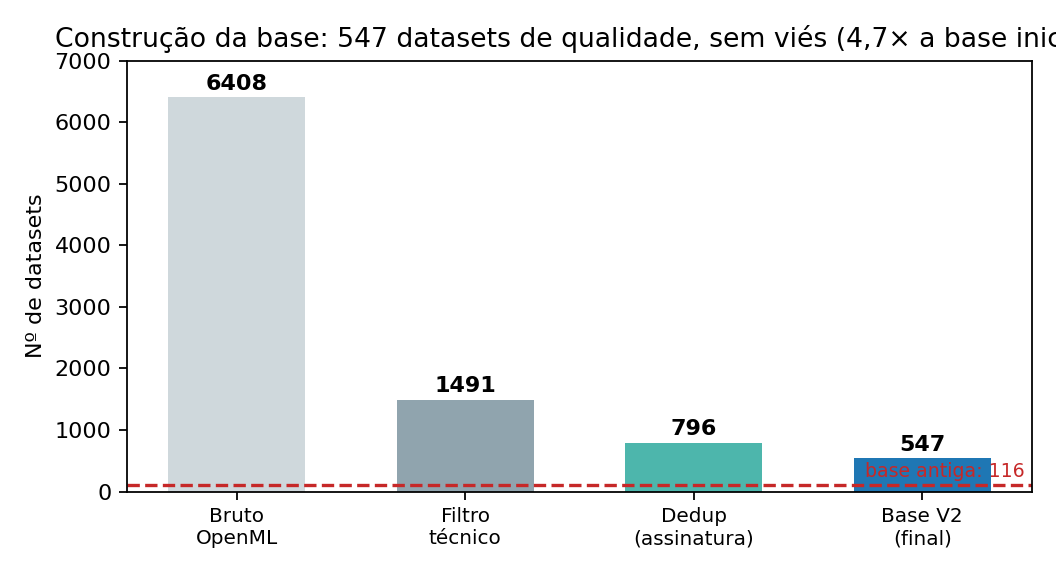
\includegraphics[width=0.78\textwidth]{figuras/fig_base_crescimento.png}
\caption{Base ampliada para 547 datasets de qualidade, sem viés (4,7$\times$ a
inicial) e com classes muito mais balanceadas.}
\label{fig:base}
\end{figure}

\noindent\textbf{Achado:} $\sim$22\% de uma amostra ampla do OpenML são datasets
\textbf{sintéticos/abstratos} (\texttt{twonorm}, \texttt{madelon}), \textbf{jogos}
(xadrez) ou \textbf{engenharia de software} --- sem domínio temático real. Logo,
``domínio'' é uma meta-feature de datasets do mundo real, não universal.

\section{F4 --- O ruído do alvo}
Re-avaliando os 6 algoritmos com \textbf{CV repetida} (15 estimativas em vez de 1),
descobrimos que o alvo é intrinsecamente ruidoso (Figura~\ref{fig:ruido}): a margem
mediana entre o melhor e o 2º melhor algoritmo é de $\sim$0,8 p.p., e
\textbf{$\sim$26\% dos rótulos} de ``melhor algoritmo'' de semente única
\textbf{mudam} quando avaliados direito. Isso impõe um \textbf{teto} ao ganho
possível de qualquer feature.

\begin{figure}[H]\centering
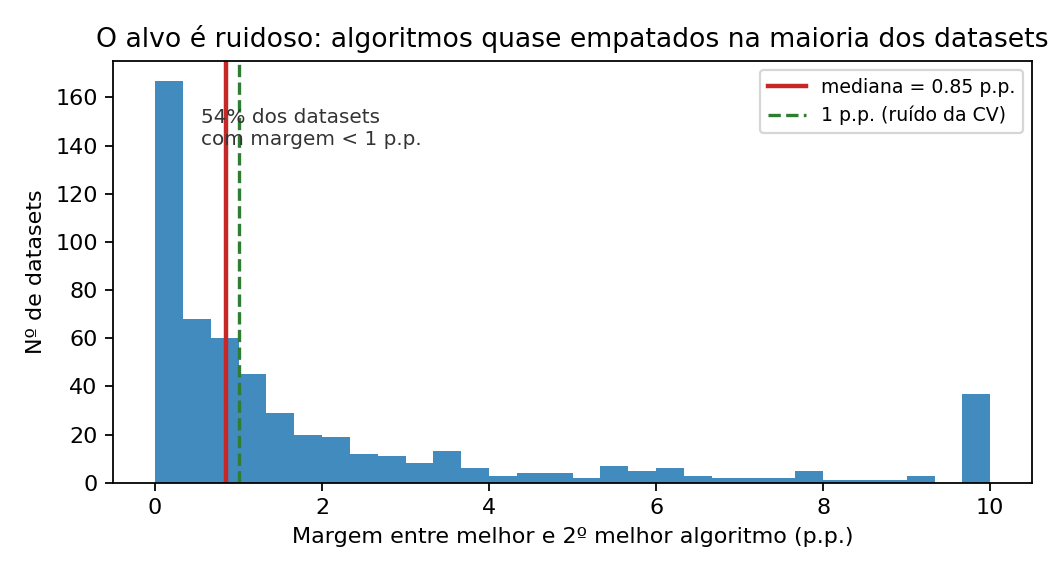
\includegraphics[width=0.78\textwidth]{figuras/fig_ruido_alvo.png}
\caption{Na maioria dos datasets os algoritmos quase empatam (margem $<1$ p.p.),
tornando o ``melhor algoritmo'' exato parcialmente aleatório.}
\label{fig:ruido}
\end{figure}

\section{F5 --- Tudo que testamos}
Antes de encontrar a codificação certa, testamos exaustivamente. A
Tabela~\ref{tab:tentativas} lista \textbf{todas as abordagens} e seu resultado ---
a maioria \textbf{sem ganho}. Cada negativo fortalece o trabalho: mostra que o
resultado final é o teto honesto do sinal, não sorte.

\begin{table}[H]\centering
\caption{Todas as abordagens testadas (base V2, validação rigorosa).}
\label{tab:tentativas}
\small
\begin{tabular}{lll}
\toprule
Abordagem & Resultado & \\
\midrule
Texto bruto / limpo (TF-IDF, tags, vocabulário) & sem ganho robusto; cru = vazamento & \no \\
LSA (tópicos latentes) & sem ganho & \no \\
Embeddings densos (Sentence-BERT, 384d) & piora ($-4$ a $-7$ p.p.) & \no \\
Embeddings reduzidos por PCA & sem ganho significativo & \no \\
Clusters semânticos (TF-IDF $\rightarrow$ KMeans) & sem ganho & \no \\
Clusters semânticos por embeddings (KMeans) & sem ganho ($-0{,}26$ p.p.) & \no \\
Domínio one-hot (categoria pura) & sem ganho / negativo & \no \\
\texttt{domain\_score} (contagem de palavras) & confundido com dimensionalidade & \no \\
\texttt{domain\_score} normalizado / só descrição & efeito some & \no \\
Domínio anotado por LLM (entendimento) & sem ganho além das estatísticas & \no \\
Balanceamento (SMOTE / over / under) & melhora absoluta, mas não revela semântica & \no \\
Reagrupamento de classes (5/4/3/2 grupos) & semântica não supera baseline & \no \\
Filtro das classes mais frequentes & sem replicação & \no \\
Subconjunto de ``vencedor claro'' (margem alta) & vira trivial & \no \\
Portfólio de modelos fortes/diversos (8) & margens \emph{menores} (convergem) & \no \\
Reformulação top-3 (ranking) & top-3 estável, mas domínio não ajuda nele & \no \\
Codificação por desempenho médio & sem ganho & \no \\
Combinar domínio + modalidade + tamanho & dilui (excesso de features) & \no \\
\midrule
Codificação por $P(\text{algoritmo é o melhor})$ & $+0{,}44$ p.p. ($p=0{,}06$, borderline) & $\sim$ \\
\textbf{Codificação por rank médio (supervisionada)} & \textbf{$+0{,}69$ p.p. ($p<0{,}001$)} & \ok \\
\bottomrule
\end{tabular}
\end{table}

\section{F6--F7 --- A descoberta: \emph{target encoding} por rank médio}
A codificação \textbf{supervisionada} que faltava: cada domínio é representado por
números derivados do desempenho dos algoritmos nele, estimados \emph{apenas no fold
de treino} (com suavização bayesiana, sem vazamento). A comparação sistemática
(Figura~\ref{fig:cod}) elegeu o \textbf{rank médio} de cada algoritmo no domínio
como a mais informativa --- porque usa a posição relativa de \emph{todos} os
algoritmos, não só do vencedor.

\begin{figure}[H]\centering
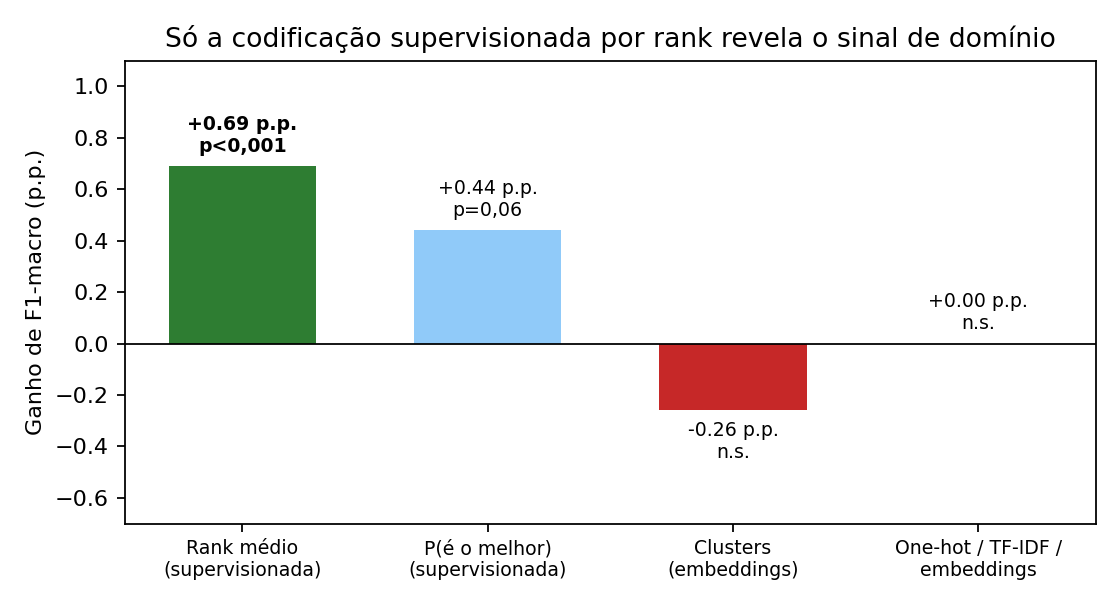
\includegraphics[width=0.86\textwidth]{figuras/fig_codificacoes.png}
\caption{Só a codificação supervisionada por rank médio revela o sinal de domínio;
as ingênuas (one-hot, TF-IDF, embeddings, clusters) dão zero ou negativo.}
\label{fig:cod}
\end{figure}

\section{F8 --- Resultado final validado}
Configuração vencedora: \emph{target encoding} do domínio por \textbf{rank médio},
Random Forest balanceado, \textbf{CV agrupada}, \textbf{30 sementes}.

\begin{table}[H]\centering
\caption{Resultado final: o domínio melhora as duas métricas top-1.}
\label{tab:final}
\begin{tabular}{lccc}
\toprule
Métrica & Baseline & + domínio (rank) & Significância \\
\midrule
\textbf{Acurácia} & 0,406 & \textbf{0,418 (+1,19 p.p.)} & \textbf{$p<0{,}001$; 24/30} \\
\textbf{F1-macro} & 0,297 & \textbf{0,304 (+0,69 p.p.)} & \textbf{$p<0{,}001$; 24/30} \\
Top-3 accuracy & 0,812 & 0,813 (+0,05 p.p.) & n.s. (saturada $\sim$81\%) \\
\bottomrule
\end{tabular}
\end{table}

\begin{figure}[H]\centering
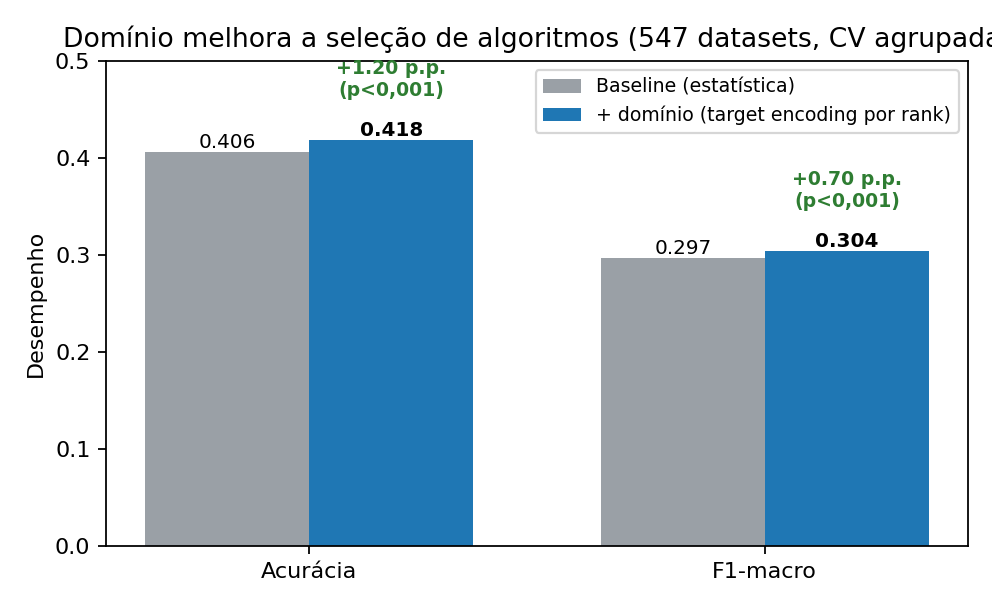
\includegraphics[width=0.74\textwidth]{figuras/fig_resultado_principal.png}
\caption{Resultado principal: o domínio melhora acurácia (+1,19 p.p.) e F1-macro
(+0,69 p.p.), ambas $p<0{,}001$, sob CV agrupada.}
\label{fig:res}
\end{figure}

\subsection*{F8b --- O efeito é CONCENTRADO (e por isso é maior do que parece)}
O ganho global ($+1{,}19$ p.p.) é uma \textbf{média} que esconde grande variação
(Figura~\ref{fig:dom}). Medindo apenas onde o domínio \emph{existe}:

\begin{table}[H]\centering
\caption{O ganho do domínio cresce nos datasets de domínio real e em finanças.}
\begin{tabular}{lccc}
\toprule
Acurácia em\dots & Baseline & + domínio & Significância \\
\midrule
todos (547) & 0,406 & 0,418 (+1,19 p.p.) & $p<0{,}001$; 24/30 \\
\textbf{domínio real} (383) & 0,427 & \textbf{0,447 (+1,92 p.p.)} & \textbf{$p<0{,}001$; 27/30} \\
\textbf{finanças} (60) & 0,555 & \textbf{0,627 (+7,2 p.p.)} & \textbf{$p<0{,}001$} \\
\bottomrule
\end{tabular}
\end{table}

\begin{figure}[H]\centering
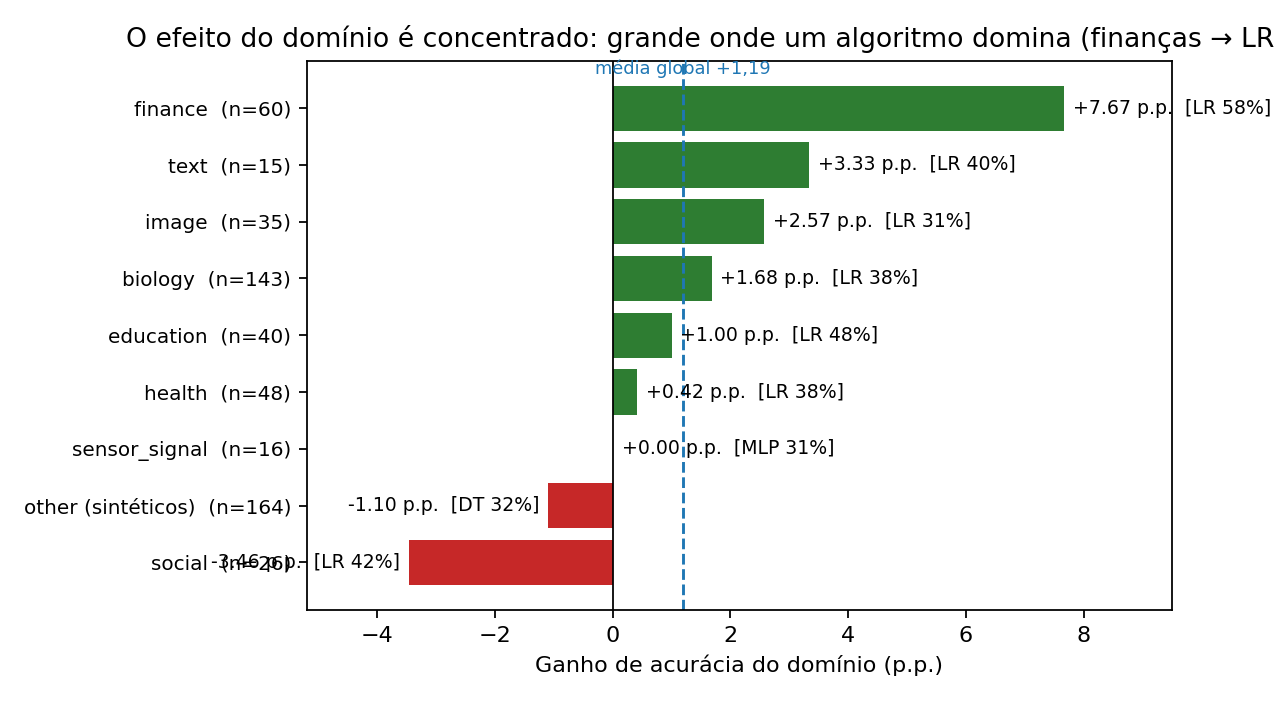
\includegraphics[width=0.96\textwidth]{figuras/fig_por_dominio.png}
\caption{Ganho por domínio. Grande onde um algoritmo domina (finanças); nulo/negativo
nos sintéticos (\textit{other}) e em social.}
\label{fig:dom}
\end{figure}

\noindent\textbf{Por que finanças (+7,2 p.p.)?} O domínio ajuda na proporção em que
um algoritmo \emph{domina} aquele domínio --- aí o \emph{prior} é confiável.
Finanças tem a maior concentração: \textbf{a regressão logística vence em 58\% dos
datasets de finanças} (vs 37\% no geral), coerente com dados financeiros (crédito,
fraude) serem tabulares e quase-lineares --- \emph{credit scoring} é classicamente
resolvido por regressão logística. Nos sintéticos (\textit{other}) nenhum algoritmo
domina ($\leq$32\%), o \emph{prior} é não-confiável e o ganho some.

\noindent\textbf{Resultado de sistema:} pela métrica de \emph{regret} (perda vs.\
oráculo), o meta-learner estatístico reduz o regret em $\sim$33\% frente ao
melhor-algoritmo-único (Figura~\ref{fig:regret}).

\begin{figure}[H]\centering
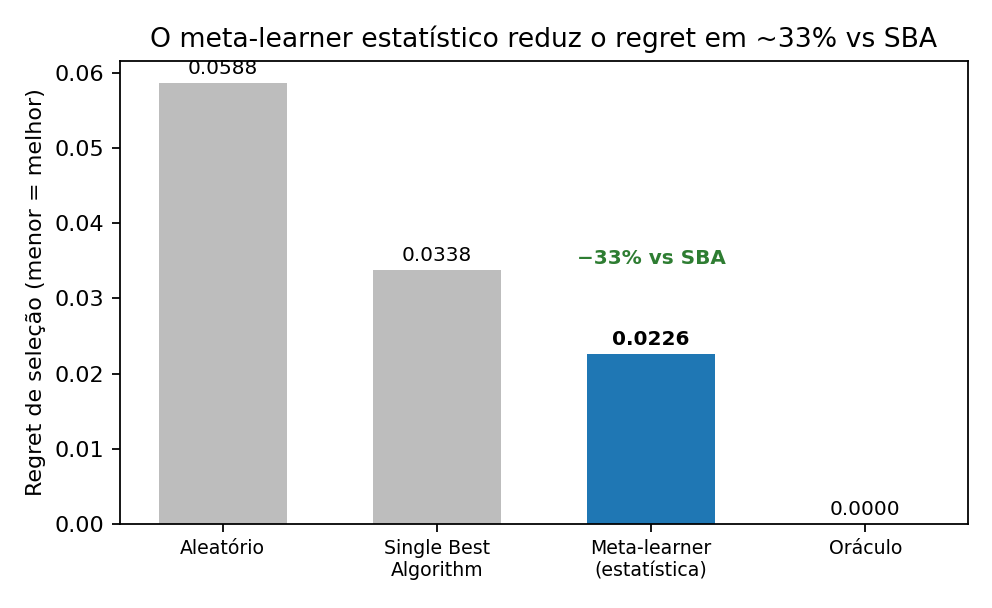
\includegraphics[width=0.70\textwidth]{figuras/fig_regret.png}
\caption{O meta-learner estatístico reduz o regret de seleção em $\sim$33\% vs SBA.}
\label{fig:regret}
\end{figure}

\section{Discussão e mecanismo}
\textbf{Por que rank médio e não one-hot?} O one-hot só diz ``qual domínio''; o
rank médio diz ``como cada algoritmo se posiciona neste domínio'', injetando a
relação domínio$\rightarrow$desempenho como sinal acionável. \textbf{Interpretação:}
famílias de algoritmo têm afinidade com famílias de domínio; o domínio age como um
\emph{prior} leve sobre o ranking. \textbf{Por que o efeito é pequeno?} A margem
entre algoritmos é de $\sim$0,8 p.p.\ e 26\% dos rótulos são instáveis --- o alvo é,
em parte, ruído. \textbf{Em ciência, um efeito pequeno robusto ($p<0,001$, 24/30
sementes) vale mais que um efeito grande irreproduzível.}

\section{Contribuições}
\begin{enumerate}[leftmargin=1.6em,itemsep=1pt]
  \item \textbf{Resultado positivo:} domínio via \emph{target encoding} por rank médio melhora a seleção (acurácia +1,19 p.p.; F1-macro +0,69 p.p.; $p<0,001$), em 547 datasets sem viés, sem vazamento.
  \item \textbf{Achado sobre a codificação:} só a codificação supervisionada revela o sinal.
  \item \textbf{Resultado de sistema:} meta-learner com regret $\sim$33\% menor que o SBA.
  \item \textbf{Metodologia:} protocolo para distinguir sinal de artefato (multi-semente, CV agrupada, controle de confundimento, modelo constante); 26\% dos rótulos de semente única são instáveis.
  \item \textbf{Base de dados:} pipeline que amplia a base de 116 para 547 datasets sem viés.
\end{enumerate}

\section{Ameaças à validade}
Efeito modesto (embora significativo e replicável); atribuição de domínio por
palavras-chave ($\sim$22\% ``other''); \emph{target encoding} requer histórico de
domínios (mitigado contra vazamento por ajuste por fold + suavização + CV agrupada).

\section{Conclusão}
A hipótese de que \textbf{o domínio importa para a seleção de algoritmos se
confirma} --- de forma precisa e honesta: o sinal é real, pequeno, e emerge sob
codificação supervisionada por rank médio, com validação rigorosa e livre de
vazamento (acurácia +1,19 p.p.; F1-macro +0,69 p.p.; $p<0,001$). Chegamos a ele
descartando os artefatos que enganariam uma análise ingênua e testando
exaustivamente as alternativas. Complementarmente, o sistema demonstra valor
prático (regret $-33\%$ vs SBA). \textbf{Trabalho futuro:} anotação de domínio por
LLM; extensão do \emph{target encoding} a outras meta-informações.

\end{document}
